\documentclass[12pt,fullpage,singlespace]{article}
\usepackage{xltxtra}
\usepackage{flushend}
\usepackage[numbers,sort&compress]{natbib}
\setmainfont{Times New Roman}

\begin{document}

\title{Chemical-Genetic Profiling and Its Applications}
\author
{
Hongjian Li\\
Department of Computer Science and Engineering\\
Chinese University of Hong Kong\\
hiji@cse.cuhk.edu.hk
}
\maketitle

\pagenumbering{arabic}

\begin{abstract}

Chemical-genetic profiling of bioactive compounds has been repeatedly proved to be a powerful tool for identifying novel drugs, mode of actions of drugs and drug targets, and for better understanding the relation between genotype and phenotype. In the past two decades, research mainly concentrated on applying chemical-genetic profiling to the yeast genome, but seldom investigated into higher organisms like mammals, or higher level of practical applications like drug synergy. This survey briefly reviews the popular experimental techniques and computational methods for constructing and analyzing chemical-genetic profiles and discusses their pros and cons. In the foreseeable future, as both the number of bioactive compounds and the number of sequenced genes increase, more and more chemical-genetic profiles will emerge. How to establish an universal database to accommodate diverse chemical-genetic output from various research groups, and how to correctly and properly utilize such ressources for better drug discovery will become challenging issues.

\end{abstract}

%\begin{IEEEkeywords}

%Chemical-Genetic Profiling, Drug-Target Pathway, Mode-of-Action

%\end{IEEEkeywords}

\section{Introduction}

Chemical genetics refers to the study of genetic responses to chemical compounds. On a genome-wide scale, it is called chemical genomics or chemogenomics. It embraces multiple early phase drug discovery technologies ranging from target identification and validation, through compound design and chemical synthesis, to biological testing and ADME profiling.

Chemical-genetic profiling is nowadays gaining more and more importance and popularity as it provides a valuable tool for a wide variety of biological applications, including but not limited to rapid identifications of novel drugs, mode of actions (MOAs) of drugs and drug targets, and understanding biological systems to a better extend by relating genotype and phenotype.

\section{Motivation}

Partly due to the massive failure of antimicrobial target-based \textit{in vitro} screening strategies over the past 20 years, chemical-genetic profiling is preferred over high-throughput screening in certain applications thanks to its ability to rapidly characterize compounds in an unbiased fashion and provide rich, functional information to elucidate their MOAs and targets.

High-throughput screening is mainly limited by two factors. The pharmaceutical targets are usually limited to a small subset of specific proteins, and it could be very difficult to conduct a comprehensive screening given the facts that the small molecule chemical space consists of as many as 10\textsuperscript{60} chemical compounds \citep{1104} and the rate of compound synthesis via combinational chemistry is constantly increasing. In contrast, chemical-genetic profiling can be genome-wide and even interspecies.

\section{Background}

Chemical-genetic profiling basically measures the quantitative values of growth defects of deletion strains under exposure to chemicals. The foundation of chemical-geneitic approach was laid with the idea to sequence the 12.5-megabase yeast \textit{Saccharomyces cerevisiae} genome in the 1980s. Figure \ref{fig:1081-1} shows the six major steps for yeast fitness profiling of pooled deletion strains. Experimental detail can be found in the original publicaton \citep{1081}. Because a deletion mutant provides a model for the effect of a compound that inhibits the gene product, genetic interaction information obtained from genome-wide synthetic lethal screens of haploid deletion mutants provides a key for interpreting chemical-genetic profiles and thereby links compounds to their target pathways based on chemical-genetic interaction data alone.

\begin{figure}
\centering
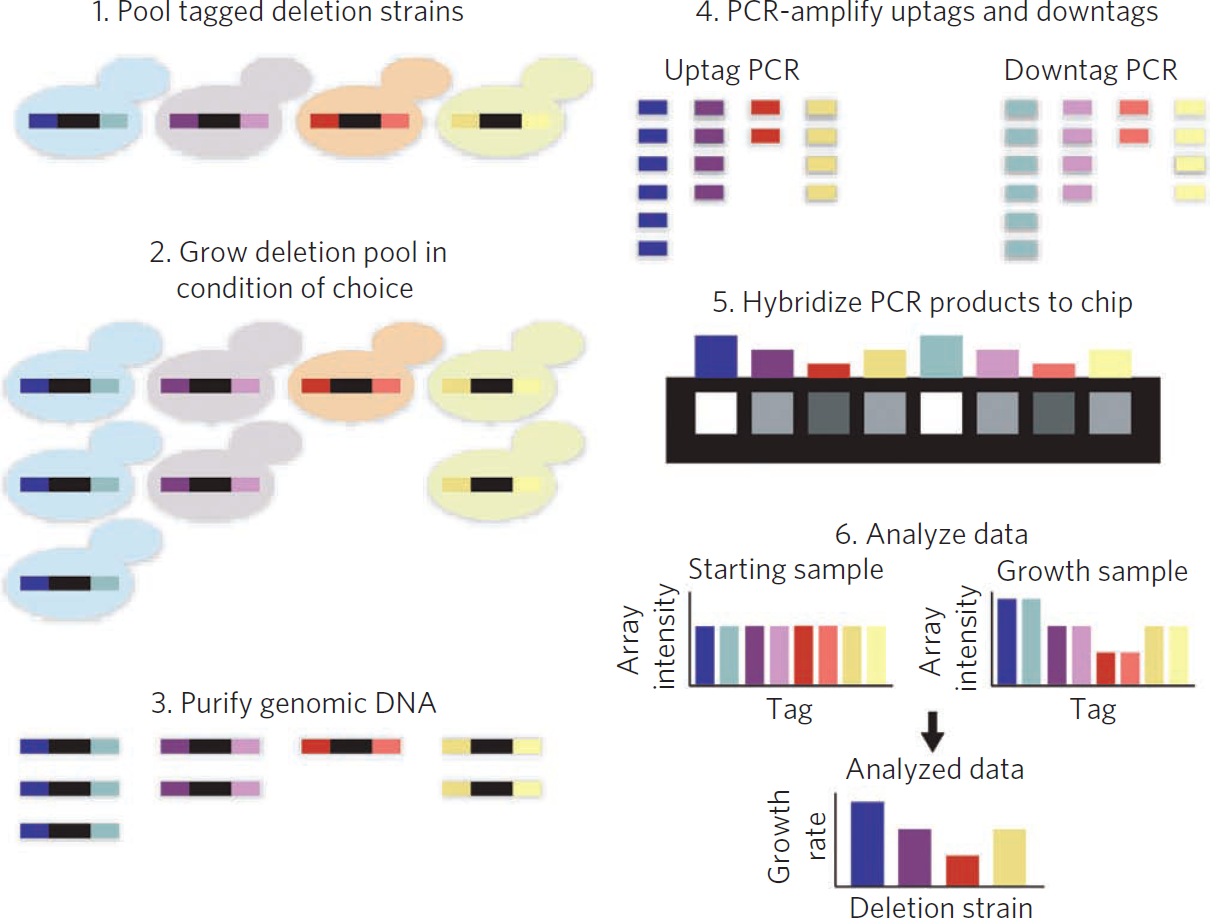
\includegraphics[width=\linewidth]{1081-1.png}
\caption{Yeast fitness profiling of pooled deletion strains. Figure reprinted from \citep{1081}.}
\label{fig:1081-1}
\end{figure}

Figure \ref{fig:1082-1} compares genetic, chemical-genetic, and chemical-chemical profiling. In the case of chemical-genetic profiling, one gene product is inactivated via gene deletion and the other is inactivated by chemical inhibition (Figure \ref{fig:1082-1}a). Red indicates a significant drug-gene interaction (Figure \ref{fig:1082-1}b). Such quantative values can be used to predict the target process of unknown agents. In the case of chemical-genetic profiling, known compounds on the X-axis are clustered based on known mode of action or function, and the Y-axis shows clustering of other unknown genes with similar profiles.

\begin{figure}
\centering
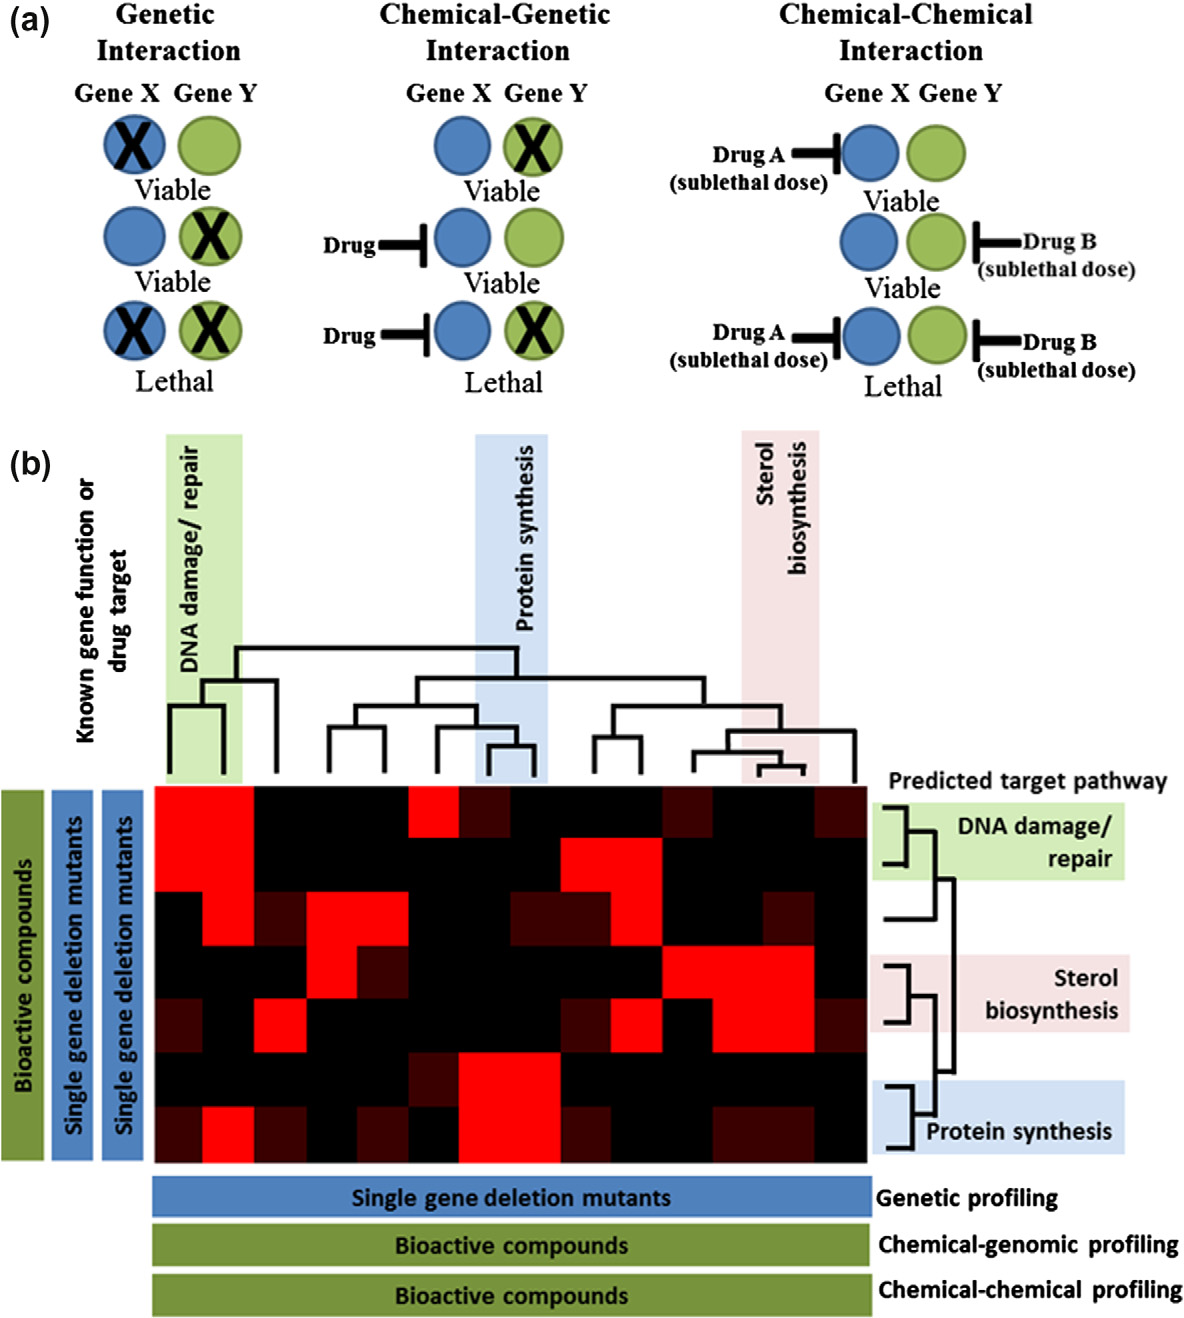
\includegraphics[width=\linewidth]{1082-1.png}
\caption{Comparison of genetic, chemical-genetic, and chemical-chemical profiling. Figure reprinted from \citep{1082}.}
\label{fig:1082-1}
\end{figure}

With the quantative interaction values produced by chemical-genetic profiling, computational methods are then applied for in-depth analysis. Popular approaches include 2D hierarchical clustering \citep{1078,1079,1080}, probabilistic sparse matrix factorization (PSMF) \citep{1078} and bayesian factor model \citep{1079}. Such algorithmic approaches could provide potentially important insight into drug-target pathway \citep{1078,1079} or address the debate concerning the purpose of nonessential genes \citep{1080}.

\section{Compendium of Chemical-Genetic Interaction}

In \citeyear{1078}, \Citeauthor{1078} generated a compendium of chemical-genetic interaction profiles by testing the collection of viable yeast haploid deletion mutants for hypersensitivity to 82 growth-inhibitory compounds and natural product extracts using parallel fitness tests of large numbers of pooled deletion strains in a minimal amount of medium thanks to the unique molecular barcodes that tag and identify each deletion strain \citep{1078}. The 82 chemical perturbations contain 75 synthetic compounds and natural products, of which 23 are FDA approved, plus 7 crude antifungal extracts, derived from different marine sponges and microorganisms. The full list and the inhibitory concentrations can be found in the original publication \citep{1078}.

Having obtained the quantative gene-drug interaction values, they then applied both a hierarchical clustering and a PSMF method, which allows a gene or compound to be associated with more than one group. Eventually they managed to find tamoxifen, a breast cancer therapeutic, to disrupt calcium homeostasis, and find phosphatidylserine as a target for papuamide B, a cytotoxic lipopeptide with anti-HIV activity.

Figure \ref{fig:1078-1} shows the results of 2D hierarchical clustering. 3,418 genes are plotted on the horizontal axis and 82 conditions are plotted on the vertical axis. Red lines indicate chemical-genetic interactions. They revealed that compounds with similar cellular effects showed similar chemical-genetic profiles and thereby cluster together on the vertical axis. They listed 11 clusters (i.e. clusters i to xi) for explanation. In cluster i, both latrunculin B and cytochalasin A are actin binding agents. In cluster ii, both staurosporine and caspofungin are cell wall synthesis inhibitors. In cluster iii, both nystatin and amphotericin act by increasing the permeability of the fungal cell membrane. These 11 examples demonstrated the power of 2D hierarchical clustering for grouping compounds known to inhibit the same pathway or target. Likewise, on the horizontal axis, deletion mutants with similar chemical sensitivities also cluster together, grouping functionally related genes.

\begin{figure}
\centering
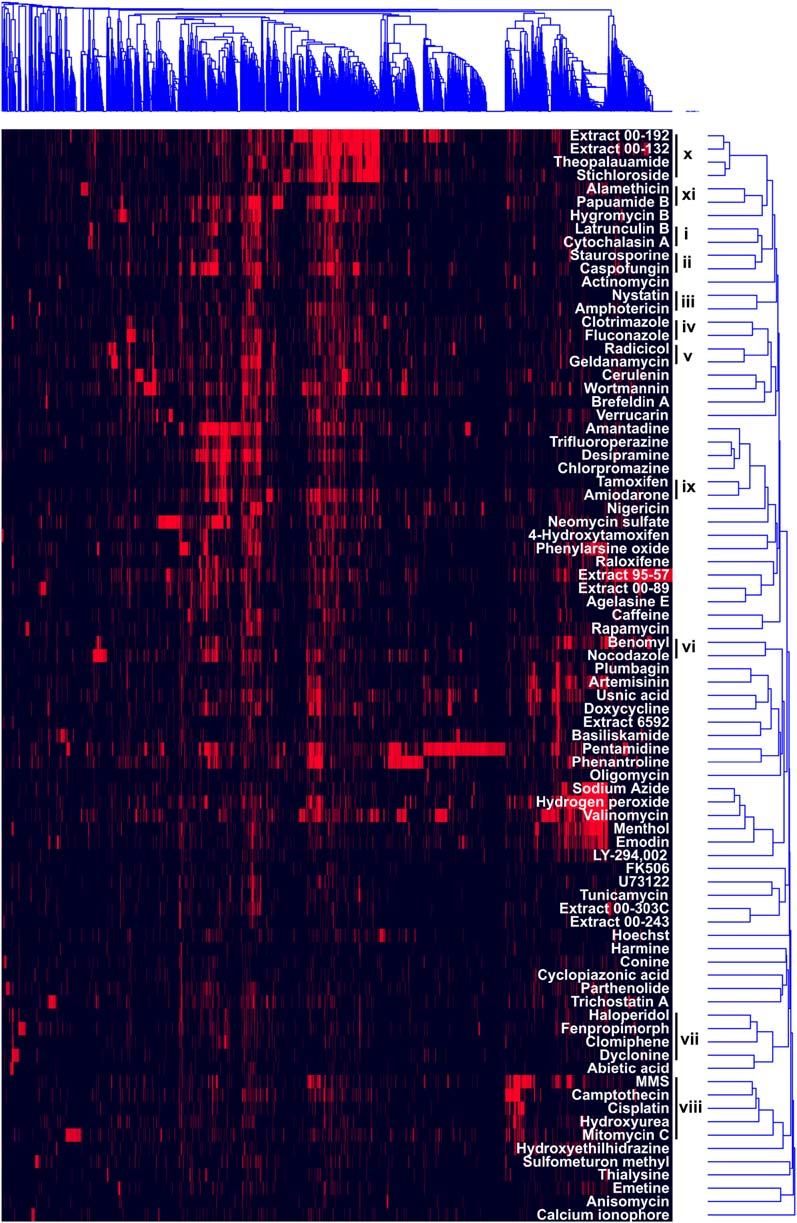
\includegraphics[width=\linewidth]{1078-1.png}
\caption{Two-dimensional hierarchical clustering analysis of chemical-genetic profiles. Figure reprinted from \citep{1078}.}
\label{fig:1078-1}
\end{figure}

The compendium can help reveal insights into the activities of human therapeutics. One particular example is cluster ix, which groups tamoxifen and amiodarone together. Tamoxifen is a competitive inhibitor of estradiol binding to the estrogen receptor and a common breast cancer drug, while amiodarone is an antianginal and antiarrhythmic drug. This cluster suggested that tamoxifen may also produce antifungal activity, which was subsequently verified and confirmed by a series of biological assays \citep{1078}.

One major limitation of 2D hierarchical clustering is its inability to associate a gene or compound with more than one group. To address this issue, the authors applied PSMF, allowing each cluster to be defined by an arbitrary set of genes and compounds (Figure \ref{fig:1078-2}). They identified 30 factors, which were referred to as subsets of compounds detected by the algorithm.

Factors 5, 6, 21 and 29 were picked out for in-depth analysis. In factor 5, papuamide B and alamethicin are the compounds that are most important in factor number 5, and this is driven by the common sensitivity of the deletion mutants listed on the y axis, with the most significant mutants at the top. Following spot dilution assays, they succeeded in linking Papuamide B, a high-molecular-weight cycliclipopeptide originally isolated from a marine sponge, to its cellular target, phosphatidylserine.

In factor 29, extract 00-192, from a sea cucumber from the Commonwealth of Dominica and extract 00-132, derived from an Indonesian marine sponge, showed highly similar chemical-genetic profiles. From the two crude extracts, antifungal compounds were purified. The two compounds do not share structural features and thus chemical-genetic profiling appears to have linked molecules with disparate chemistry to the same biological activity.

\begin{figure}
\centering
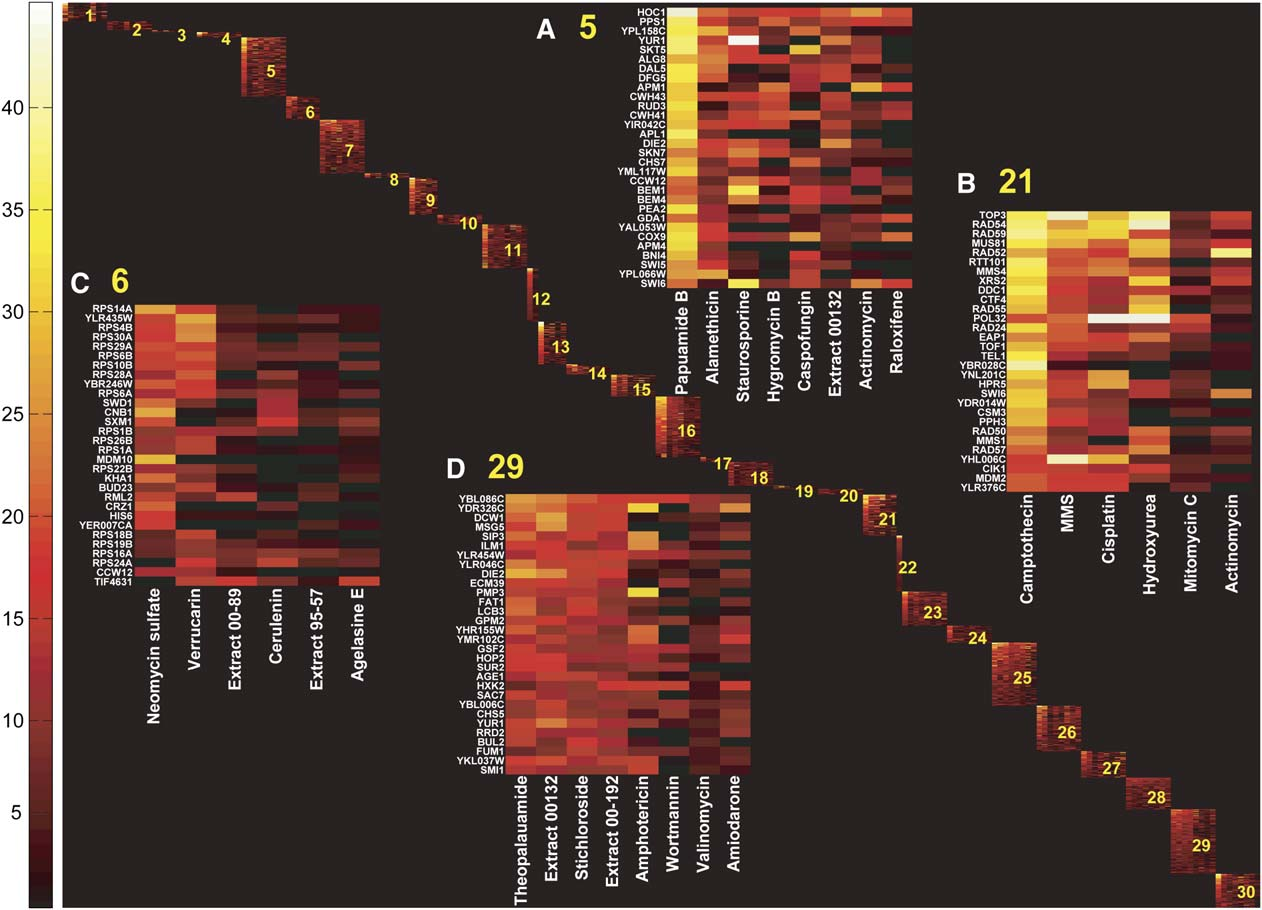
\includegraphics[width=\linewidth]{1078-2.png}
\caption{Visualization of results from PSMF. Figure reprinted from \citep{1078}.}
\label{fig:1078-2}
\end{figure}

\section{Protein Complex-Based Bayesian Factor Model}

The profiles in the previous study \citep{1078} have not been yet modeled at the molecular level in terms of biological real entity such as protein complexes. Inspired by the desire to overcome this issue, in \citeyear{1079}, \Citeauthor{1079} exploited the same compendium of chemical-genetic interaction but incorporated protein-protein and genetic interactions as additional valuable biological information \citep{1079}. They assumed protein complexes (PCs) were functional units for yeast cell growth and regarded them as hidden factors and developed the PC-based Bayesian factor model that relates the chemical-genetic profile at the level of organism phenotypes to the hidden activities of PCs at the molecular level (Figure \ref{fig:1079-1}). This assumption comes from the basic idea that the observed growth fitness measurements of each strain are determined by combined effects of the activities of PCs in each cell in a given treatment.

\begin{figure}
\centering
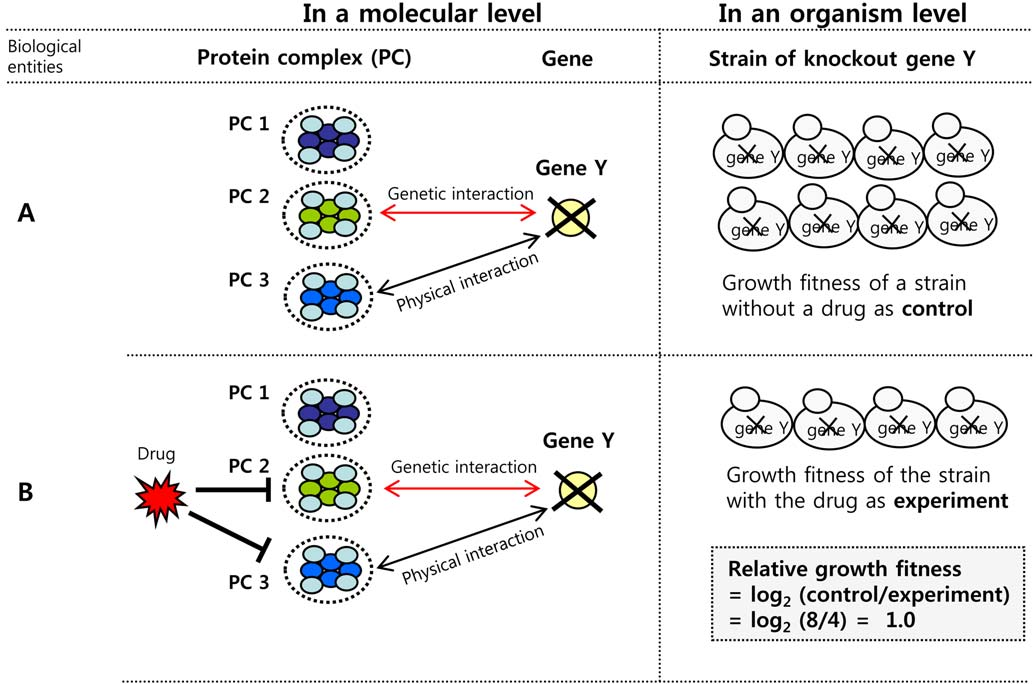
\includegraphics[width=\linewidth]{1079-1.png}
\caption{Model assumption on protein complexes as hidden factors underlying fitness of strain. Figure reprinted from \citep{1079}.}
\label{fig:1079-1}
\end{figure}

Figure \ref{fig:1079-2} depicts the Bayesian inference procedures. The bipartite network of 488 protein complexes and 4,111 strains (Figure \ref{fig:1079-2}a) was abstracted into a binary association matrix (i.e. Z matrix). Both the Z matrix and the chemical-genetic profiles (i.e. E matrix) (Figure \ref{fig:1079-2}b) were input to Protein Complex-based Bayesian factor Analysis (PCBA), which yielded as output both the relative protein complex activities under chemicals and relative growth fitness of strains under chemicals (Figure \ref{fig:1079-2}c).

\begin{figure}
\centering
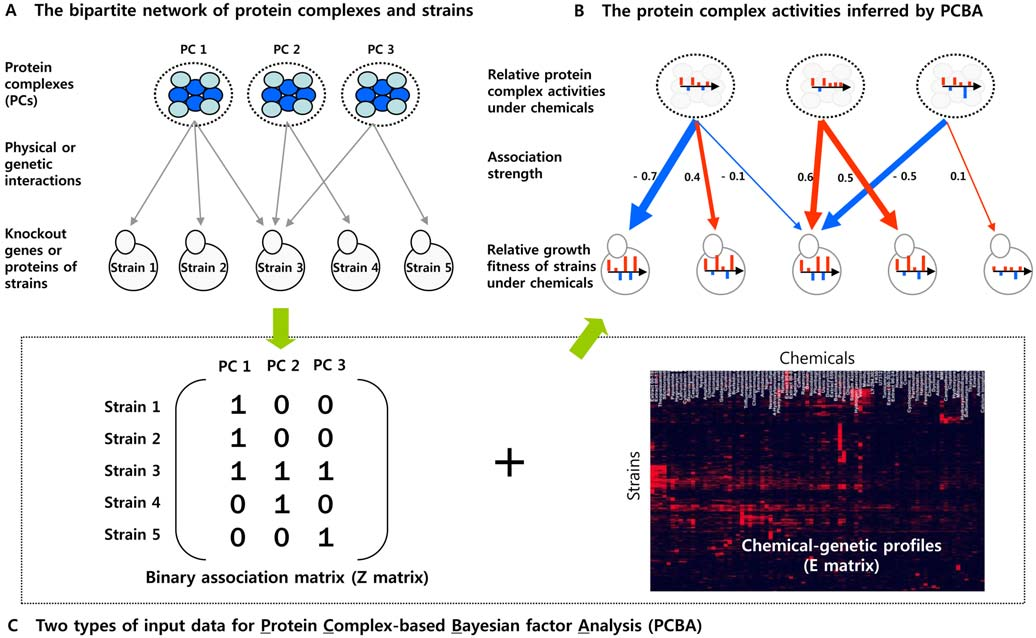
\includegraphics[width=\linewidth]{1079-2.png}
\caption{Procedures for inferring the hidden activities of a collection of protein complexes in a cell. Figure reprinted from \citep{1079}.}
\label{fig:1079-2}
\end{figure}

Similarly, the authors performed 2D hierarchical clustering (Figure \ref{fig:1079-3}). However, instead of plotting genes on the X axis and chemicals on the Y axis, in this PC-based case they plotted 82 drugs on the X axis and 488 proteins on the Y axis, claiming that such integration of prior knowledge helped to reduce the large dimension of chemical-genetic profiles (4111 by 82) into relatively small dimension of chemical-PC profiles (488 by 82) in a biologically meaningful way. Among the 14 clusters (i.e. a to n), 9 were similarly predicted in both dendrograms. For the rest 5 clusters, the authors surveyed relevant literature evidences and claimed their clustering results were more reliable, and gave possible reasons for their improvement.

\begin{figure}
\centering
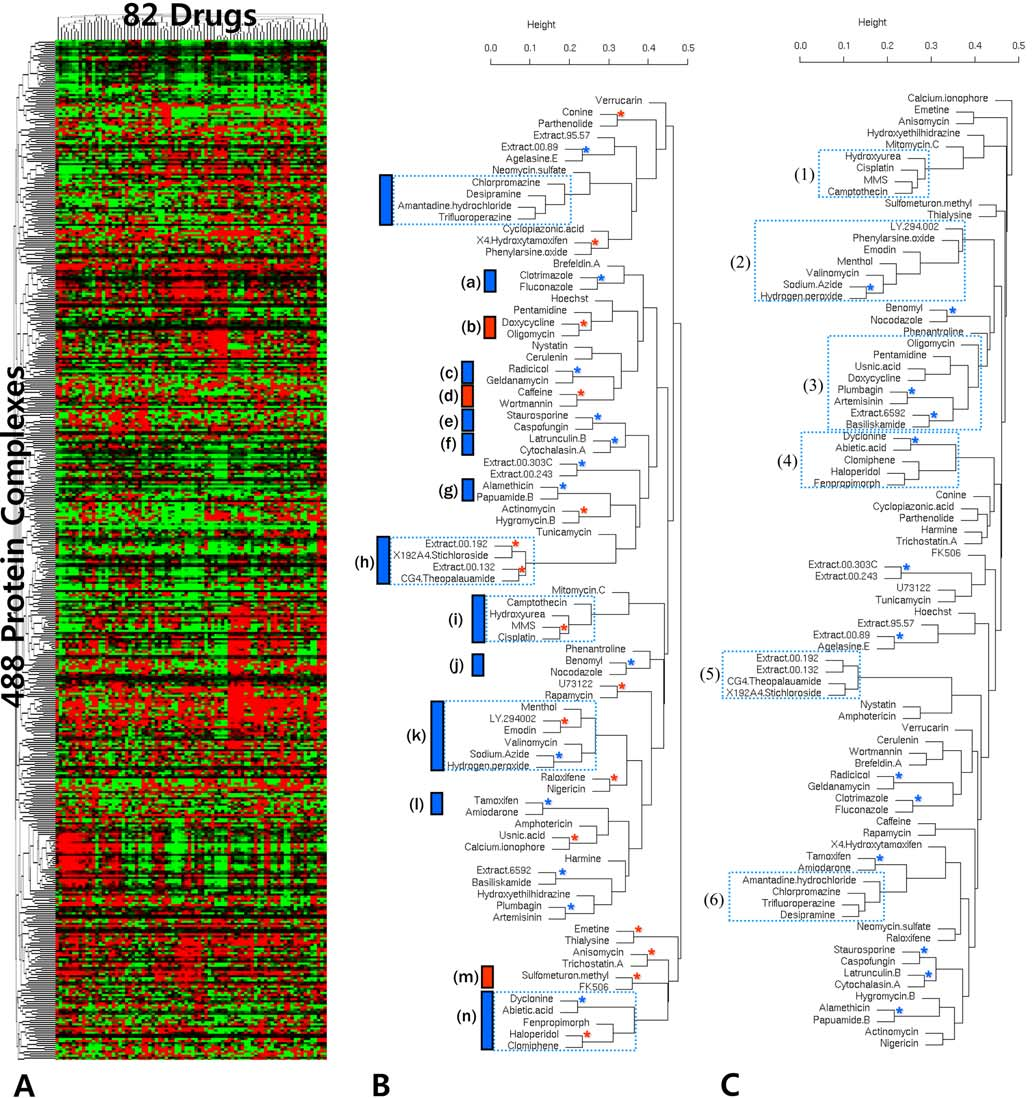
\includegraphics[width=\linewidth]{1079-3.png}
\caption{Clustering analysis of protein complex activities. (A) Bird eyes of 2D hierarchical clustering. (B) The PC-based hierarchical dendrogram of 82 drugs using relative activities of all of 488 protein complexes as performed in \citep{1079}. (C) The strain-based hierarchical dendrogram of 82 drugs using the growth fitness of 3,418 strains as performed in \citep{1078}. Figure modified from \citep{1079}.}
\label{fig:1079-3}
\end{figure}

From the chemical-PC hierarhical clustering results, the authors argued that their complex-based clusters (Figure \ref{fig:1079-3}B) showed more physiologically meaningful grouping of drugs compared with strain-based clusters (Figure \ref{fig:1079-3}C) in yeast. They used as an example sulfometuron methyl and FK506, which are very different chemicals in their structures, by both of which the same physiological effect of branched amino acid depletion occurs in yeast. Moreover, they were able to highlight TOR1 as the target protein of rapamycin from cluster I and topoisomerase I as the target protein of camptothecin from cluster III (Figure \ref{fig:1079-4}). Even further, they could predict the MOAs of rapamycin (Figure \ref{fig:1079-5}) and camptothecin.

\begin{figure}
\centering
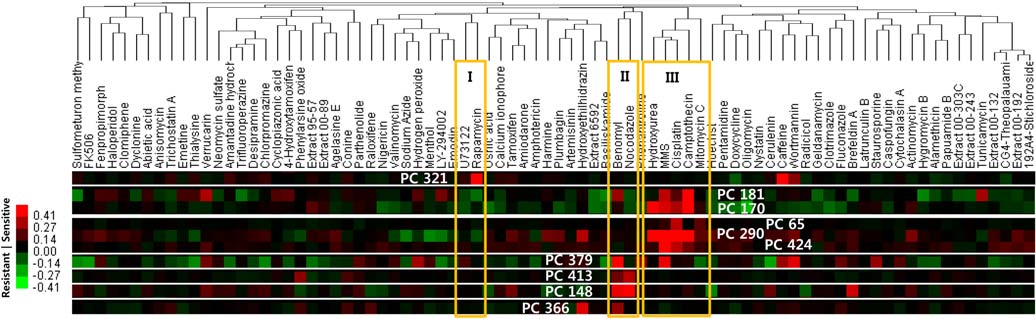
\includegraphics[width=\linewidth]{1079-4.png}
\caption{Significantly sensitive protein complexes to drugs known for their target pathway. Figure reprinted from \citep{1079}.}
\label{fig:1079-4}
\end{figure}

\begin{figure}
\centering
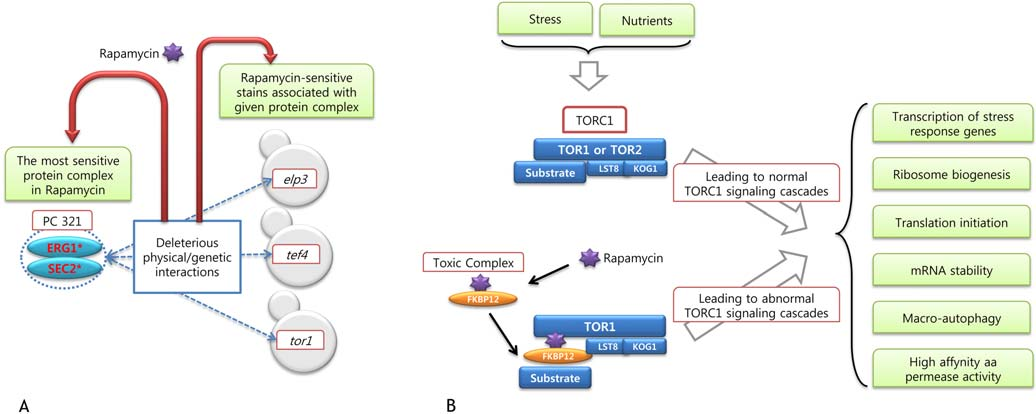
\includegraphics[width=\linewidth]{1079-5.png}
\caption{Target pathway of rapamycin. Figure reprinted from \citep{1079}.}
\label{fig:1079-5}
\end{figure}

\section{Discussion}

The completion of the 12.5-megabase yeast genome sequencing in the 1980s laid the foundation of chemical-genetic profiling. Ever since, chemical-genetic profiling began to gradually capture the attention of molecular biologists, thanks to its power for rapid identifications of novel drugs, MOAs and drug targets in a comprehensive manner. In \citeyear{1078}, \Citeauthor{1078} generated a compendium of chemical-genetic interaction. Two years later, \Citeauthor{1079} proposed a protein complexed-based Bayesian factor model, integrating the compendium as well as biological interaction network as additional information. Both groups managed to shed light on MOAs of certain drugs. In the same year, \Citeauthor{1080} performed 1,144 heterozygous deletion experiments and 418 homozygous deletion experiments on the yeast whole-genome deletion collections and quantified the growth fitness of each deletion strain in the presence of chemical or environmental stress conditions \citep{1080}. They claimed to find 97\% of gene deletions exhibite a measurable growth phenotype, suggesting nearly all genes are essential for optimal growth in at least one condition, addresses the debate concerning the purpose of nonessential genes. \Citeauthor{1103} composed a tutorial on chemical genetics \citep{1103}, explaining relevant concepts and highlighting recent developments in four areas of biology, including small molecule modulation of protein-protein interactions (PPIs), \textit{plasmodium falciparum}, hepatitis C virus and RNA interference pathways.

1081 review key discoveries that gave rise to the field of chemical genetics, with particular attention to chemical-genetic strategies developed for bakers’ yeast, their extension to clinically relevant microbial pathogens, and the potential of these approaches to affect antimicrobial drug discovery.

1082 review CG profiling, focusing on emerging cross-species technologies and novel drug-synergy applications, as well as outlining needs within the field.

1080 it suggests that virtually the entire genome is conditionally essential and therefore accessible to inhibition with small molecules. The study also showed that more than 500 genes (12\% of the genome) behave as multidrug-resistance (MDR) genes


1078 This study also highlighted the fact that some cellular processes are particularly sensitive to compound perturbation and that clustering of sensitivity profiles can aid in assigning MOA to previously uncharacterized compounds.

Key component of the model is Z matrix (binary association matrix), which not only allowed us to robustly compute the equation, but also provided a window through which relevant biological information such as protein-protein interactions and genetic interactions can be integrated with experimental data.

the estimation of protein complex activities by Bayesian factor model is more robust and stable because estimands are obtained by tens of thousands of samplings.

Z matrix too coarse. PSMF is suitable in case of no prior knowledge.

the inferred results are biologically interpretable, which allowed us to develop an effective way to predict drug’s target pathway.


Our PC-based approach would not properly work if too many numbers of insufficient and incorrect components of protein complexes are used as hidden factors to represent whole dynamic cellular events and also insufficient and incorrect biological interactions are integrated for the associations between PC and strains in our model. In that case, some true positives of drug-target genes would be lost.

In current study, we used only chemical-genetic profiles of about 5,000 viable yeast haploid mutants as observed data for our modeling. It means that the effect of any of the about 1,000 essential genes to a bioactive compound was not able to be included as observations.


Prior to clustering, we processed the data by removing a set of 121 genes whose corresponding deletion mutant displayed statistically significant multidrug sensitivity. investigated in \citep{1080}

have only cataloged 2\%-4\% of all genetic interactions and so our ability to integrate chemical-genetic and genetic interaction data is limited

In my opinion, the complicated and biased barcode-based chemical-genetic profiling procedures constitute the bottleneck in the whole picture. Many compounds are in limited supply, and thus a major challenge is to screen the collection of yeast deletion mutants efficiently. Parallel fitness tests were employed in \citep{1078}.

State-of-the-art genome deletion project \citep{1107}

Despite the advantages of the reverse chemical-genetic strategies described here, substantial time and effort are required to construct such resources. 

the mouse conditional KO collection a predicted 3 years from completion,43 mammalian CG profiling will likely become a more straightforward assay \citep{1082}.

experimental cost, researchers must choose the most appropriate method to maximize resource-to-result ratio.

\section{Prospectives}

In the future, two achievements can be possibly expected. They are a centralized and open source repository for chemical-genetic data, and high-level applications with advanced statistical methods and diverse biological knowledge.

The need to establish a universal repository for effectively and efficiently warehousing and accessing the huge amount of emerging chemical-genomic data is aroused recently given the hundreds of sequenced organisms including mammals. Since the chemical-genetic profiling experiments were done by different research groups worldwide using different biological assays under different environmental conditions, it would be challenging to appropriately remove the bias and absord them into a single central database for public access. One successful example is the Protein Data Bank (PDB) \citep{105}, which collects very diverse macromolecular structures resolved by X-ray crystallography, nuclear magnetic resonance or other technologies. Another successful example is the ZINC database \citep{532}, which integrates drug-like, lead-like and fragment-like ligands from various academic and commercial sources.

Another trend is to apply sophisticated statistical models and computer algorithms and utilize more types of available biological data in order to really solve high-level drug discovery problems, like drug synergy, where the combined effect of two drugs exceeds the expected sum of the individual agents. The previous study \citep{1078}  generated a compendium of chemical-genetic interaction and made use of it for MOA prediction. They subsequent study \citep{1079} combined the compendium together with the bipartite network of protein complexes and strains and utilized the more robust PCBA approach for drug-target pathway prediction. Following this trend, it is straightforward to see such diverse biological knowledge as drug ADME profiles, gene ontologies, genetic interactions, protein-protein interactions, protein-chemical interactions, transcriptional regulatory network and so on being incorporated into a universal high-dimensional computational method for high-level predictions.

In conclusion, as both the number of bioactive compounds and the number of sequenced genes increase, how to construct an universal database to accommodate diverse output from various research groups, and how to correctly and properly utilize such ressources for better drug discovery are likely to become challenging issues in the foreseeable future.

\bibliographystyle{unsrtnat}
\bibliography{../refworks}

\end{document}
